\documentclass{standalone}
\usepackage[T1]{fontenc}
\usepackage[latin2]{inputenc}
\usepackage[english]{babel}
\usepackage{tikz}
\usepackage{times}
\usetikzlibrary{calc,through,backgrounds,positioning,fit}
\usetikzlibrary{shapes,arrows,shadows}
 
\begin{document}
 
 
\centering
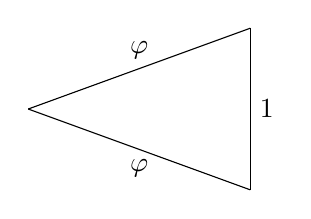
\begin{tikzpicture}

\draw (0,0) -- (20:3) coordinate (p1)node[color=black,above, pos=0.5] {$\varphi$};
\draw (0,0) -- (340:3) coordinate (p2)node[color=black,below, pos=0.5] {$\varphi$};;

\draw (p1) -- (p2)node[color=black,right, pos=0.5] {$1$};;

\end{tikzpicture}

 
\end{document}